\documentclass[12pt]{article}
%% Packages
\usepackage{amssymb}
\usepackage{amsmath}
\usepackage{amsthm}
\usepackage{amsfonts}
\usepackage{mathtools}
\usepackage{xspace}
\usepackage{bm}
\usepackage{nicefrac}
\usepackage{bbm}
\usepackage{boxedminipage}
\usepackage{xparse}
\usepackage[x11names]{xcolor}
\usepackage{float}
\usepackage{multirow}
\usepackage{graphicx}
\usepackage{caption}
\usepackage{subcaption}
\usepackage{ifthen}
\usepackage{algpseudocode}
%\usepackage{algorithmic}
\usepackage{array}
\usepackage{wrapfig}
\usepackage{geometry}
%\usepackage{enumitem}
\usepackage{pgfplots}


\usepackage{tikz}
\usetikzlibrary{positioning}
\usetikzlibrary{fit}
\usetikzlibrary{calc}
\usetikzlibrary{backgrounds}
\usetikzlibrary{shapes}
\usetikzlibrary{patterns}
\usetikzlibrary{matrix}
\usetikzlibrary{intersections}

\usepackage[pdftex,bookmarks=true,pdfstartview=FitH,colorlinks,linkcolor=blue,filecolor=blue,citecolor=blue,urlcolor=blue,pagebackref=true]{hyperref}
    \urlstyle{sf}
    
% No figures taking up one whole page
\renewcommand{\floatpagefraction}{.8}%

%% Document Design Choices
%\setlength{\parindent}{0pt}
%\setlength{\parskip}{10pt}
%\renewcommand{\labelitemi}{\ensuremath{\circ}}
\geometry{left=1in, right=1in, top=1in, bottom=1in}
\makeatletter
\renewcommand{\paragraph}{%
	\@startsection{paragraph}{4}%
	{\z@}{4pt \@plus 0pt \@minus 0pt}{-1em}%
	{\normalfont\normalsize\bfseries}%
}
\makeatother


%% Marking
\newcommand\TODO[1]{{\color{red}{#1}}\xspace}

%% Theorems and Environments
%
%\makeatletter
%\newtheorem*{rep@theorem}{\rep@title}
%\newcommand{\newreptheorem}[2]{%
%\newenvironment{rep#1}[1]{%
% \def\rep@title{\theoremref{##1} Restated}%
% \begin{rep@theorem}}%
% {\end{rep@theorem}}}
%\makeatother
%
%\makeatletter
%\newtheorem*{rep@lemma}{\rep@title}
%\newcommand{\newreplemma}[2] {%
%\newenvironment{rep#1}[1]{%
% \def\rep@title{\lemmaref{##1} Restated}%
% \begin{rep@lemma}}%
% {\end{rep@lemma}}}
%\makeatother
%
\newtheorem{theorem}{Theorem}
%\newreptheorem{theorem}{Theorem}
\newtheorem{importedlemma}{Imported Lemma}
\newtheorem{importedtheorem}{Imported Theorem} 
%\newtheorem{informaltheorem}{Informal Theorem}
\newtheorem{definition}{Definition}
\newtheorem{lemma}{Lemma}
\newtheorem{proposition}{Proposition}
%\newreplemma{lemma}{Lemma}
\newtheorem{claim}{Claim}
\newtheorem{corollary}[theorem]{Corollary}
\newtheorem{observation}{Observation}


\newenvironment{boxedalgo}
  {\begin{center}\begin{boxedminipage}{\linewidth}}
  {\end{boxedminipage}\end{center}}


%% References
\newcommand{\namedref}[2]{\hyperref[#2]{#1~\ref*{#2}}\xspace}
\newcommand{\lemmaref}[1]{\namedref{Lemma}{lem:#1}}
\newcommand{\propref}[1]{\namedref{Proposition}{prop:#1}}
\newcommand{\theoremref}[1]{\namedref{Theorem}{thm:#1}}
\newcommand{\claimref}[1]{\namedref{Claim}{clm:#1}}
\newcommand{\corolref}[1]{\namedref{Corollary}{corol:#1}}
\newcommand{\figureref}[1]{\namedref{Figure}{fig:#1}}
\newcommand{\tableref}[1]{\namedref{Table}{tbl:#1}}
\newcommand{\equationref}[1]{\namedref{Equation}{eq:#1}}
\newcommand{\defref}[1]{\namedref{Definition}{def:#1}}
\newcommand{\observationref}[1]{\namedref{Observation}{obs:#1}}
\newcommand{\procedureref}[1]{\namedref{Procedure}{proc:#1}}
\newcommand{\importedtheoremref}[1]{\namedref{Imported Theorem}{impthm:#1}}
\newcommand{\informaltheoremref}[1]{\namedref{Informal Theorem}{infthm:#1}}

\newcommand{\sectionref}[1]{\namedref{Section}{sec:#1}}
\newcommand{\appendixref}[1]{\namedref{Appendix}{app:#1}}


%% English
\newcommand{\ie}{\text{i.e.}\xspace}
\newcommand{\st}{\text{s.t.}\xspace}
\newcommand{\etal}{\text{et al.}\xspace}
\newcommand{\naive}{\text{na\"ive}\xspace}
\newcommand{\wrt}{\text{w.r.t.}\xspace}
\newcommand{\whp}{\text{w.h.p.}\xspace}
\newcommand{\resp}{\text{resp.}\xspace}
\newcommand{\eg}{\text{e.g.}\xspace}
\newcommand{\cf}{\text{cf.}\xspace}
\newcommand{\visavis}{\text{vis-\`a-vis}\xspace}
\newcommand{\aka}{\text{a.k.a.}\xspace}


%% Names
\newcommand{\gacs}[0]{G\'acs\xspace}
\newcommand{\korner}[0]{K\"orner\xspace}
\newcommand{\turan}[0]{Tur{\'a}n\xspace}
\newcommand{\erdos}[0]{Erd\H{o}s\xspace}


%% Crypto
\def\alice{{{Alice}}\xspace}
\def\bob{{{Bob}}\xspace}
\def\eve{{{Eve}}\xspace}
%\newcommand{\poly}{\ensuremath{\mathrm{poly}}\xspace}
\DeclareMathOperator{\poly}{poly}
\DeclareMathOperator{\polylog}{polylog}
\newcommand{\negl}{\ensuremath{\mathsf{negl}}\xspace}
\newcommand{\secpar}{\ensuremath{{\kappa}}\xspace}
\newcommand{\zo}{\ensuremath{{\{0,1\}}}\xspace}

  %% Protocol Tree
  \def\Achildren{\mathsf{AliceChildren}}
  \def\Bchildren{\mathsf{BobChildren}}
  \def\Echildren{\mathsf{EveChildren}}
  
  %% Functionalities
  \newcommand{\func}[1]{\ensuremath{\cF_{\mathsf{#1}}}\xspace}
  \newcommand{\fcom}[0]{\func{com}}
  \newcommand{\fot}[0]{\func{ot}}
  
  %% Protocols
  % \newcommand{\prot}[1]{\ensuremath{\pi_{\mathsf{#1}}}\xspace}


%% Graph Theory
\newcommand{\ancest}[0]{\mathsf{Ancestors}}
\newcommand{\sibling}[0]{\mathsf{Siblings}}
\newcommand{\parent}[0]{\mathsf{parent}}
\newcommand{\leaves}[0]{\mathsf{leaves}}


%% Math Symbols
\renewcommand{\o}[0]{\ensuremath{\circ}\xspace}
\newcommand{\dist}[1]{\ensuremath{\left\langle{#1}\right\rangle}\xspace}
\newcommand{\prob}[2]{\ensuremath{\dist{{#1}_1, \dotsc, {#1}_{#2}}}\xspace}
\newcommand{\ip}[2]{\ensuremath{\left\langle{#1},{#2}\right\rangle}\xspace}
\renewcommand{\vec}[1]{\ensuremath{\mathbf{#1}}\xspace}
\newcommand{\concat}[0]{\ensuremath{\circ}\xspace}
\newcommand{\nin}[0]{\ensuremath{\not\in}\xspace}
\newcommand{\xor}[0]{\ensuremath{\oplus}\xspace}
\newcommand{\rv}[1]{\ensuremath{\mathbf{#1}}\xspace}
\newcommand{\p}[1]{\ensuremath{^{{\left(#1\right)}}}\xspace}
\newcommand{\argmax}[0]{\ensuremath{\mathop{\mathrm{argmax}}\;}\xspace}
\newcommand{\argmin}[0]{\ensuremath{\mathop{\mathrm{argmin}}\;}\xspace}
\newcommand{\maj}[0]{\ensuremath{\mathop{\mathrm{maj}}\;}\xspace}
\NewDocumentCommand\mathstack{>{\SplitList{;}}m}
  {\ensuremath{
    \begin{smallmatrix}
      \ProcessList{#1}{ \insertone }    
    \end{smallmatrix}
  }}
\newcommand{\insertone}[1]{\ensuremath{#1}\\}

%\newcommand{\argmax}{\operatornamewithlimits{argmax}}
%\DeclareMathOperator*{\argmax}{arg\,max}

  
  %% General
  \newcommand{\ceil}[1]{\ensuremath{\left\lceil{#1}\right\rceil}\xspace}
  \newcommand{\floor}[1]{\ensuremath{\left\lfloor{#1}\right\rfloor}\xspace}
  \newcommand{\abs}[1]{\ensuremath{\left\vert{#1}\right\vert}\xspace}
  \newcommand{\lone}[1]{\ensuremath{\left\vert{#1}\right\vert}\xspace}
  \newcommand{\spnorm}[1]{\ensuremath{\left\Vert{#1}\right\Vert}\xspace}

  %% Renamed Symbols
  \newcommand{\eps}[0]{\ensuremath{\varepsilon}}
  \let\epsilon\eps
  
  %% Cal Alphabets
  \newcommand{\cA}{\ensuremath{{\mathcal A}}\xspace}
  \newcommand{\cB}{\ensuremath{{\mathcal B}}\xspace}
  \newcommand{\cC}{\ensuremath{{\mathcal C}}\xspace}
  \newcommand{\cD}{\ensuremath{{\mathcal D}}\xspace}
  \newcommand{\cE}{\ensuremath{{\mathcal E}}\xspace}
  \newcommand{\cF}{\ensuremath{{\mathcal F}}\xspace}
  \newcommand{\cG}{\ensuremath{{\mathcal G}}\xspace}
  \newcommand{\cH}{\ensuremath{{\mathcal H}}\xspace}
  \newcommand{\cL}{\ensuremath{{\mathcal L}}\xspace}
  \newcommand{\cM}{\ensuremath{{\mathcal M}}\xspace}
  \newcommand{\cN}{\ensuremath{{\mathcal N}}\xspace}
  \newcommand{\cO}{\ensuremath{{\mathcal O}}\xspace}
  \newcommand{\cP}{\ensuremath{{\mathcal P}}\xspace}
  \newcommand{\cQ}{\ensuremath{{\mathcal Q}}\xspace}
  \newcommand{\cR}{\ensuremath{{\mathcal R}}\xspace}
  \newcommand{\cS}{\ensuremath{{\mathcal S}}\xspace}
  \newcommand{\cT}{\ensuremath{{\mathcal T}}\xspace}
  \newcommand{\cU}{\ensuremath{{\mathcal U}}\xspace}
  \newcommand{\cV}{\ensuremath{{\mathcal V}}\xspace}
  \newcommand{\cW}{\ensuremath{{\mathcal W}}\xspace}
  \newcommand{\cX}{\ensuremath{{\mathcal X}}\xspace}
  \newcommand{\cY}{\ensuremath{{\mathcal Y}}\xspace}
  \newcommand{\cZ}{\ensuremath{{\mathcal Z}}\xspace}
  
  %% Bold Alphabets
  \newcommand{\bA}{\ensuremath{{\mathbf A}}\xspace}
  \newcommand{\bB}{\ensuremath{{\mathbf B}}\xspace}
  \newcommand{\bC}{\ensuremath{{\mathbf C}}\xspace}
  \newcommand{\bD}{\ensuremath{{\mathbf D}}\xspace}
  \newcommand{\bE}{\ensuremath{{\mathbf E}}\xspace}
  \newcommand{\bF}{\ensuremath{{\mathbf F}}\xspace}
  \newcommand{\bG}{\ensuremath{{\mathbf G}}\xspace}
  \newcommand{\bQ}{\ensuremath{{\mathbf Q}}\xspace}
  \newcommand{\bU}{\ensuremath{{\mathbf U}}\xspace}
  \newcommand{\bV}{\ensuremath{{\mathbf V}}\xspace}
  \newcommand{\ba}{\ensuremath{{\mathbf a}}\xspace}
  \newcommand{\be}{\ensuremath{{\mathbf e}}\xspace}
  \renewcommand{\bm}{\ensuremath{{\mathbf m}}\xspace}
  \newcommand{\br}{\ensuremath{{\mathbf r}}\xspace}
  \newcommand{\bs}{\ensuremath{{\mathbf s}}\xspace}
  \newcommand{\by}{\ensuremath{{\mathbf y}}\xspace}  
    
  %% Black-board Bold Alphabets
  \newcommand{\bbA}{\ensuremath{{\mathbb A}}\xspace}
  \newcommand{\bbB}{\ensuremath{{\mathbb B}}\xspace}
  \newcommand{\bbC}{\ensuremath{{\mathbb C}}\xspace}
  \newcommand{\bbD}{\ensuremath{{\mathbb D}}\xspace}
  \newcommand{\bbE}{\ensuremath{{\mathbb E}}\xspace}
  \newcommand{\bbF}{\ensuremath{{\mathbb F}}\xspace}
  \newcommand{\bbG}{\ensuremath{{\mathbb G}}\xspace}
  \newcommand{\bbH}{\ensuremath{{\mathbb H}}\xspace}
  \newcommand{\bbI}{\ensuremath{{\mathbb I}}\xspace}
  \newcommand{\bbJ}{\ensuremath{{\mathbb J}}\xspace}
  \newcommand{\bbK}{\ensuremath{{\mathbb K}}\xspace}
  \newcommand{\bbN}{\ensuremath{{\mathbb N}}\xspace}
  \newcommand{\bbO}{\ensuremath{{\mathbb O}}\xspace}
  \newcommand{\bbP}{\ensuremath{{\mathbb P}}\xspace}
  \newcommand{\bbQ}{\ensuremath{{\mathbb Q}}\xspace}
  \newcommand{\bbR}{\ensuremath{{\mathbb R}}\xspace}
  \newcommand{\bbS}{\ensuremath{{\mathbb S}}\xspace}
  \newcommand{\bbT}{\ensuremath{{\mathbb T}}\xspace}
  \newcommand{\bbV}{\ensuremath{{\mathbb V}}\xspace}
  \newcommand{\bbZ}{\ensuremath{{\mathbb Z}}\xspace}
  
  %% Fraktur Alphabets
  \newcommand{\fP}{\ensuremath{{\mathfrak P}}\xspace}
  \newcommand{\fR}{\ensuremath{{\mathfrak R}}\xspace}
  \newcommand{\fX}{\ensuremath{{\mathfrak X}}\xspace}
  
  %% Hat Alphabets
  \newcommand{\he}{\ensuremath{\widehat{e}}\xspace}
  \newcommand{\hf}{\ensuremath{\widehat{f}}\xspace}
  \newcommand{\hn}{\ensuremath{\widehat{n}}\xspace}
  \newcommand{\hv}{\ensuremath{\widehat{v}}\xspace}
  \newcommand{\hw}{\ensuremath{\widehat{w}}\xspace}
  \newcommand{\hx}{\ensuremath{\widehat{x}}\xspace}
  \newcommand{\hy}{\ensuremath{\widehat{y}}\xspace}
  \newcommand{\hz}{\ensuremath{\widehat{z}}\xspace}
  
  \newcommand{\hG}{\ensuremath{\widehat{G}}\xspace}
  \newcommand{\hI}{\ensuremath{\widehat{I}}\xspace}
  \newcommand{\hO}{\ensuremath{\widehat{O}}\xspace}
  
  %% Tilde Alphabets
  \newcommand{\tC}{\ensuremath{\widetilde{C}}\xspace} 
  \newcommand{\tO}{\ensuremath{\widetilde{O}}\xspace} 
  
  \newcommand{\tm}{\ensuremath{\widetilde{m}}\xspace} 
  
  \newcommand{\talpha}{\ensuremath{\widetilde{\alpha}}\xspace} 
  
  %% Fractions
  \newcommand{\half}{\ensuremath{\frac12}\xspace}
  
  %% Set
  \newcommand{\comp}[1]{\ensuremath{\overline{{#1}}}\xspace}
  
  %% Models
  \newcommand{\defeq}[0]{\ensuremath{{\;\vcentcolon=\;}}\xspace}
  \newcommand{\eqdef}[0]{\ensuremath{{\;=\vcentcolon\;}}\xspace}
  \newcommand{\entails}[0]{\ensuremath{{\models}}\xspace}
  
  %% Matrix
  \newcommand{\tran}[0]{\ensuremath{^{\mathsf{T}}}\xspace}
  
  %% Probability and Distributions
  \newcommand{\event}[1]{\ensuremath{\mathsf{#1}}\xspace}
  \newcommand{\supp}[0]{\ensuremath{\mathsf{Supp}}\xspace}
  \newcommand{\pr}[0]{\mathop{\mathrm{Pr}}\xspace}
  %\renewcommand{\Pr}[0]{\mathrm{\generateerror}\xspace}
  \newcommand{\E}[0]{\mathop{\bbE}\xspace}
  \newcommand{\getsr}[0]{\mathbin{\stackrel{\mbox{\,\tiny \$}}{\gets}}}
  \newcommand{\drawn}{\ensuremath{\sim}\xspace}
  %\newcommand{\sd}[2]{\ensuremath{\mathbf{\Delta}\left({#1},{#2}\right)}\xspace}
  \newcommand{\sd}[2]{\ensuremath{\mathrm{SD}\left(\;{#1}\;,\;{#2}\;\right)}\xspace}
  \newcommand{\iid}[0]{\text{i.i.d.}\xspace}
  
    %% Random Variables
    \newcommand{\rvA}{\rv{A}}
    \newcommand{\rvB}{\rv{B}}
    \newcommand{\rvC}{\rv{C}}
    \newcommand{\rvD}{\rv{D}}
    \newcommand{\rvL}{\rv{L}}
    \newcommand{\rvP}{\rv{P}}
    \newcommand{\rvQ}{\rv{Q}}
    \newcommand{\rvR}{\rv{R}}
    \newcommand{\rvS}{\rv{S}}
    \newcommand{\rvT}{\rv{T}}
    \newcommand{\rvU}{\rv{U}}
    \newcommand{\rvV}{\rv{V}}
    \newcommand{\rvW}{\rv{W}}
    \newcommand{\rvX}{\rv{X}}
    \newcommand{\rvY}{\rv{Y}}
    \newcommand{\rvZ}{\rv{Z}}
    
    \newcommand{\rvm}{\rv{m}}
    \newcommand{\rvr}{\rv{r}}
    \newcommand{\rvx}{\rv{x}}
    \newcommand{\rvy}{\rv{y}}

  %% Binary Operators
  \newcommand{\band}[0]{\ensuremath{~\wedge~}\xspace}
  \newcommand{\bor}[0]{\ensuremath{~\vee~}\xspace}
  \let\leq\leqslant
  \let\geq\geqslant
  
  %% Combinatorial
  \renewcommand\choose[2]{\ensuremath{{
    \left(\begin{matrix}
      {#1}\\
      {#2}
    \end{matrix}\right)}}\xspace}
  \newcommand{\fact}[1]{\ensuremath{{#1}!}\xspace}
  \newcommand\gchoose[3]{\ensuremath{{
    \left[\begin{matrix}
      {#1}\\
      {#2}
    \end{matrix}\right]\ifthenelse{\equal{#3}{}}{}{_{#3}}
  }}\xspace} 
  
  %% Set Operations
  \newcommand{\union}[0]{\ensuremath{\cup}\xspace}
  \newcommand{\intersect}[0]{\ensuremath{\cap}\xspace}
  \newcommand{\setdiff}[0]{\ensuremath{\Delta}\xspace}
  

%% Algorithms, Predicates
\newcommand{\pred}[1]{\ensuremath{\mathsf{#1}}\xspace}

\newcolumntype{L}[1]{>{\raggedright\let\newline\\\arraybackslash\hspace{0pt}}m{#1}}
\newcolumntype{C}[1]{>{\centering\let\newline\\\arraybackslash\hspace{0pt}}m{#1}}
\newcolumntype{R}[1]{>{\raggedleft\let\newline\\\arraybackslash\hspace{0pt}}m{#1}}


%% Local Terms
\usepackage{mathrsfs}
\usepackage{relsize}
\usetikzlibrary{arrows}

\newcommand{\sub}[1]{\ensuremath{_{[#1]}}\xspace}
\newcommand{\supb}[1]{\ensuremath{^{[#1]}}\xspace}

% command for IP matrix in text
%\newcommand{\IP}[2]{\ensuremath{\mathsf{IP}_{{#1}\ifthenelse{\equal{#2}{}}{}{,{#2}}}}\xspace}

\newcommand{\VS}[2]{\ensuremath{\mathsf{VS}_{\ifthenelse{\equal{#1}{}}{k}{#1}, \ifthenelse{\equal{#2}{}}{n}{#2}}}\xspace}

% command for Template matrix
\newcommand{\TMP}[3]{\ensuremath{\mathsf{Template}_{#1}\left(#2,#3\right)}\xspace}

% commands for G and H matrix
\newcommand{\smat}[3]{\ensuremath{#1_{#2}\p{#3}}\xspace}

% base case environment and referencing
%\newtheorem*{basecase}{Base Case}

\makeatletter
\newcommand{\manuallabel}[2]{\def\@currentlabel{#2}\label{#1}}
\makeatother

\newcommand{\baseref}[1]{\namedref{Base Case}{base:#1}}

% command for simple decomposition
\newcommand{\DCMP}[1]{\ensuremath{\mathsf{DCMP}\left(#1\right)}\xspace}

% entropy commands

\newcommand{\entropy}{\ensuremath{\mathbf{H}}\xspace}

% min-entropy
\newcommand{\minentropy}[1][]{\ensuremath{\mathbf{H_\infty}\ifthenelse{\equal{#1}{}}{}{\left(#1\right)}}\xspace}

% average min-entropy
\newcommand{\ame}[1][] {\ensuremath{\mathbf{\widetilde{H}_\infty}\ifthenelse{\equal{}{#1}}{}{\left(#1\right)}}\xspace}

% span command
\newcommand{\myspan}[1]{\ensuremath{\pred{span}\left\langle {#1} \right\rangle}\xspace}

% DS distribution
\newcommand{\DS}[1]{\ensuremath{\cD_{#1}}\xspace}

% uniform
\newcommand{\unif}[1]{\ensuremath{U_{\zo^{\ifthenelse{\equal{#1}{}}{}{#1}}}}\xspace}

% GF command
\newcommand{\GF}[1]{\ensuremath{\bbG\bbF\left[#1\right]}\xspace}


% simple partition number command
\newcommand{\simp}[1]{\ensuremath{\pred{sp}\left(#1\right)}\xspace}

% leaky correlation
\newcommand{\leaky}[2]{\ensuremath{\left({#1}\right)^{[#2]}}\xspace}

% OT hybrid
\newcommand{\OT}[1][]{\ensuremath{%
  \pred{OT}%
    \ifthenelse{\equal{#1}{}}%
      {}%
      {^{#1}}%
}\xspace}

% OLE hybrid
\newcommand{\OLE}[1][]{\ensuremath{%
  \pred{OLE}%
    \ifthenelse{\equal{#1}{}}%
      {}%
      {\left({#1}\right)}%
}\xspace}

% ROT correlation
\newcommand{\ROT}[1][]{\ensuremath{%
  \pred{ROT}%
    \ifthenelse{\equal{#1}{}}%
      {}%
      {^{#1}}%
}\xspace}

% IP correlation
\newcommand{\IP}[1][]{\ensuremath{%
  \pred{IP}%
    \ifthenelse{\equal{#1}{}}%
      {}%
      {\left({#1}\right)}%
}\xspace}

% ROLE correlation
\newcommand{\ROLE}[1][]{\ensuremath{%
  \pred{ROLE}%
    \ifthenelse{\equal{#1}{}}%
      {}%
      {\left({#1}\right)}%
}\xspace}

% bp
\newcommand{\bp}[1]{\ensuremath{\pred{bp}\left(#1\right)}\xspace}

% sp
\renewcommand{\sp}[1]{\ensuremath{\pred{sp}\left(#1\right)}\xspace}

% Inner Product
\newcommand{\inp}[2]{\ensuremath{\langle {#1},{#2} \rangle}\xspace}

% Really widehat
\usepackage{scalerel,stackengine}
\stackMath
\newcommand\reallywidehat[1]{%
	\savestack{\tmpbox}{\stretchto{%
			\scaleto{%
				\scalerel*[\widthof{\ensuremath{#1}}]{\kern-.5pt\bigwedge\kern-.5pt}%
				{\rule[-\textheight/2]{1.5ex}{\textheight}}%WIDTH-LIMITED BIG WEDGE
			}{\textheight}% 
		}{0.5ex}}%
	\stackon[1pt]{#1}{\tmpbox}%
}


\newcommand{\tn}{\ensuremath{\widetilde n}\xspace}
\newcommand{\tA}{\ensuremath{\widetilde A}\xspace}
\newcommand{\tB}{\ensuremath{\widetilde B}\xspace}
\newcommand{\tX}{\ensuremath{\widetilde X}\xspace}
\newcommand{\tZ}{\ensuremath{\widetilde Z}\xspace}

% command for commenting blocks
\newif\ifcomment
\commentfalse

\newcommand{\LPN}{\ensuremath{\pred{LPN}}\xspace}


\usepackage[T1]{fontenc}


\begin{document}




\def\majiemail{hmaji@cs.purdue.edu}
\def\haiemail{nguye245@cs.purdue.edu}
\def\alexemail{block9@cs.purdue.edu}
\author{
  Alexander R. Block%
  \thanks{
	  Department of Computer Science,
	  Purdue University.
	  \href{mailto:\alexemail}{$\mathtt{\alexemail}$}.
  }\and 
  Hemanta K. Maji%
  \thanks{
    Department of Computer Science,
    Purdue University.
    \href{mailto:\majiemail}{$\mathtt{\majiemail}$}.
  }\and
  Hai H. Nguyen%
  \thanks{
	  Department of Computer Science,
	  Purdue University.
	  \href{mailto:\haiemail}{$\mathtt{\haiemail}$}.
  } 
}


\title{Hardness Results for Simple Partition Number}

\date{\today}

\maketitle

\TODO{We wish to submit this to ISIT 2019 (deadline: January 13, 2019).
Towards this, we have the following goals for Simple Partition Number.
\begin{enumerate}
	\item Show formally that computing a simple partition is NP-hard/complete.
	In particular, we can consider first the decision problem of whether or not a graph $G$ has a simple partition of size at most $2$, and try to show this problem is NP-hard/complete.
	Starting with bipartite graphs and maybe trying to show for general graphs.
	
	\item Formally prove \theoremref{reduction} below.
	This will show we have a quartic, non-convex program for computing sp which will always terminate to an integer solution.
	
	\item Try to generalize our program and/or hardness reduction to weighted sp or other variants of sp.
	
	\item Try to show hardness of approximation of sp, similar to that of bp.
	
	\item Give at least one or two applications of sp.
	Recall example of $n$ students needing to meet with some $m$ teachers in one big room, minimize number of hours required, or something of the like.
\end{enumerate}}

\pagestyle{empty}
\thispagestyle{empty}

%\input{abstract}

\newpage
\newlength{\temp}
\setlength{\temp}{\parskip}
\setlength{\parskip}{.4\parskip}
\tableofcontents
\setlength{\parskip}{\temp}

\newpage
\setcounter{page}{1}
\pagestyle{plain}

\newpage
\section{Non-linear, Non-convex Programming}
In this section, we are interested in formulating the simple partition number of a graph $ G $ as a programming optimization problem. \\
We can formulate the simple partition number problem as a graph coloring problem. Every edge has a unique color such that edges with the same color form a simple subgraph. We want to minimize the number of colors needed. Given a graph $ G = (L, R, E)$, it is trivial to see that the number of colors needed is at most $ \abs{E(G)} $. The informal formulation is as following. 
\begin{enumerate}
	\item Suppose we are given a set of $ k $ colors $ \{1, 2, \cdots , k \} $. Note that $ k $ is fixed. For each $  i \in [k] $, let $ y^i \in \zo $ be an indicator random variable for the event that the color $ i $ has been used in coloring. 
	\item For each edge $ e \in E(G) $ and each $ i \in [k] $, let $ x_e^i \in \zo $ be an indicator random variable for the event that the edge $ e $ has color $ i $. Note that since every edge has a unique color, $ \sum\limits_{i = 1}^k x_e^i = 1 $. 
	\item Any edge with color $ i $ implies that the color $ i $ has been used, i.e, $ x_e^i \leq y^i $. 
	\item We want to make sure that the edges with the same color  form a simple subgraph $ G $. For any $ i \in [k]$, $ u, u' \in L $ and $ v, v' \in R  $, we have 
	$$(x_{u,v}^i + x_{u',v'}^i) (x_{u,v'}^i + x_{u',v}^i)( x_{u,v}^i \cdot x_{u', v'}^i - x_{u, v'}^i \cdot x_{u', v}^i) = 0 $$
\end{enumerate}
Here is an integer programming formulation with variables $ y^i $ and $ x_e^i $. 

minimize $ \sum\limits_{i =1}^k y^i $ 

subject to 
\begin{enumerate}
	\item $ y^i \in \{0,1 \} $ for every $ i \in [k] $
	\item $ x_e^i \in \{ 0,1 \} $ for every $  i \in [k] $, $  e \in E(G) $
	\item $ \sum\limits_{i =1}^k x_e^i = 1 $ for every $  i \in [k] $, $  e \in E(G) $
	\item $ x_e^i \leq y^i $ for every $  i \in [k] $, $  e \in E(G) $
	\item $(x_{u,v}^i + x_{u',v'}^i) (x_{u,v'}^i + x_{u',v}^i)( x_{u,v}^i \cdot x_{u', v'}^i - x_{u, v'}^i \cdot x_{u', v}^i) = 0 $ for every $ u, v\in L $ and $ u', v' \in R $
\end{enumerate}
note that this program is quartic (degree 4) and is not convex. We can relax this integer program to a real-number program by relaxing the second constraint, namely, $ 0 \leq x_e^i  \leq 1 $ for every $  i \in [k] $, $  e \in E(G) $. We are interested in whether the integer programing and the relaxed programming have the same optimal value or not. 




\newpage
\section{Reduction of General sp to Integer Optimal Solution}

\begin{figure}[htp]
\begin{center}

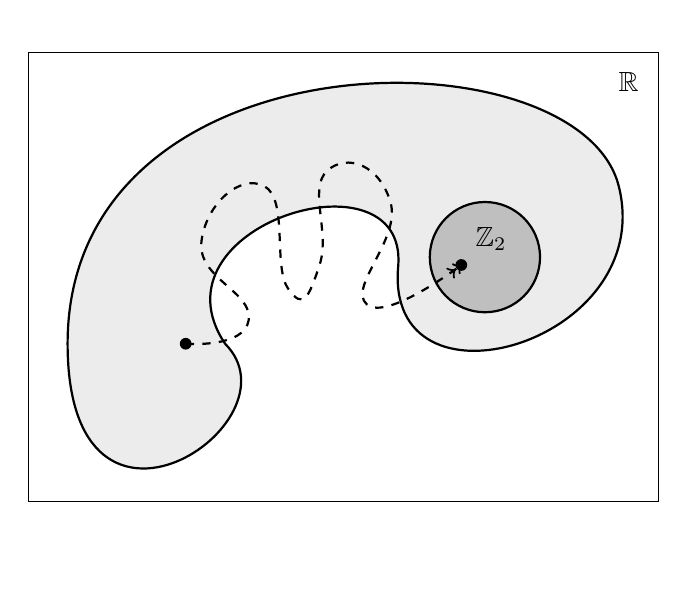
\begin{tikzpicture}

% help grid
\draw[draw] (-0.5,1) rectangle (7.5,6.7);
\node[label={below left:$\bbR$}] at (7.5,6.7) {};

%%% Bezier curves for bean shape %%%
\draw[thick, fill=gray!15] (0,3) .. controls (0,7) and (6.5,7)  ..  (7,5) .. controls (7.5,3) and (4,2) ..  (4.2,4) .. controls (4.3,5.5) and (1,4.5) .. (2,3).. controls (3,2) and (0,0) .. (0,3);
%% end bezier curves for bean shape %%%

% integer solution circle
\draw[thick, fill=gray!50] (5.3,4.1) circle (.7cm);
% point inside the circle
\node[inner sep = 1.5pt, black, circle, fill, label={above right:$\bbZ_2$}] at (5,4) (circP){};

% point inside bean
\node[inner sep = 1.5pt, black, circle, fill] at (1.5,3) (beanP) {};

% path from beanP to circP
%\draw[gray] (beanP) -- (2.3,3.3) -- (1.7,4.3) -- (2.5,5) -- (2.8,3.7) -- (3.2,4) -- (3.3,5.2) -- (4.1,4.8) -- (3.8,3.5) -- (circP);
\draw[dashed, thick, ->>] plot [smooth, tension=1] coordinates {(beanP) (2.3,3.3) (1.7,4.3) (2.5,5) (2.8,3.7) (3.2,4) (3.3,5.2) (4.1,4.8) (3.8, 3.5) (circP)};


%\iffalse
%% command to help see bezier curves
%\newcommand\DrawPoint[3]{
%	%	\node[#2,circle,fill=#2,inner sep=2pt,label={above:{\footnotesize$#1$}},label={[black]below:{\footnotesize#3}}] at #1 {}
%}
%%%% Bezier curves for bean shape %%%
%\draw[thick] (0,3) .. controls (0,7) and (6.5,7)  ..  (7,5)
%\DrawPoint{(0,3)}{red}{}
%\DrawPoint{(7,5)}{red}{}
%\DrawPoint{(0,7)}{blue}{1}
%\DrawPoint{(6.5,7)}{blue}{2}
%;
%
%\draw[thick] (7,5) .. controls (7.5,3) and (4,2) ..  (4.2,4)
%\DrawPoint{(4.2,4)}{red}{}
%\DrawPoint{(7.5,3)}{blue}{1}
%\DrawPoint{(4,2)}{blue}{2}
%;
%
%\draw[thick] (4.2,4) .. controls (4.3,5.5) and (1,4.5) .. (2,3)
%\DrawPoint{(2,3)}{red}{}
%\DrawPoint{(4.4,5.5)}{blue}{1}
%\DrawPoint{(1,4.5)}{blue}{2}
%;
%
%\draw[thick] (2,3) .. controls (3,2) and (0,0) .. (0,3)
%\DrawPoint{(3,2)}{blue}{1}
%\DrawPoint{(0,0)}{blue}{2}
%;
%%%% end bezier curves for bean shape %%%
%\fi
\end{tikzpicture}

\end{center}
\caption{An intuitive picture of how our algorithm proceeds. The path denotes the steps of the algorithm. Note that at any intermediate step, the current solution of the algorithm may not be within the space of solutions.}
\end{figure}

\begin{figure}[htp]
\begin{center}
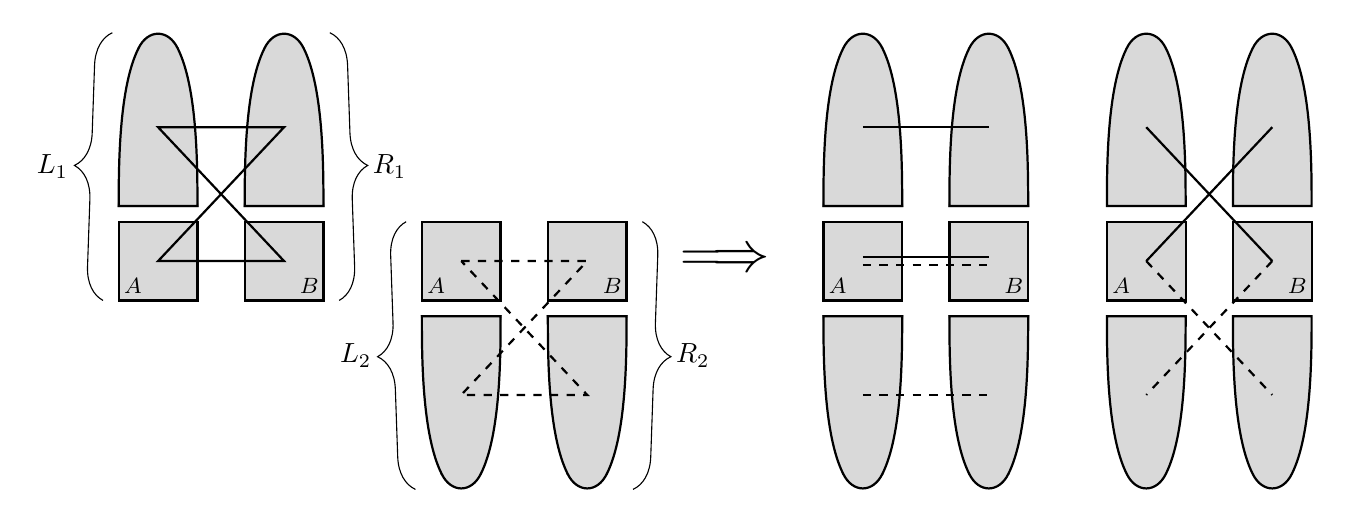
\begin{tikzpicture}

% Command for creating top shape. First 4 arguments expect
% 4 vertices of the form:
% 	(x,y), (x+.25,y+2), (x+.75,y+2), (x+1,y) 
% The 5th argument is the outline color, and the 6th
% argument is the fill color.
\newcommand{\mytop}[6]{
\draw[thick, color=#5, fill=#6] (#1) .. controls ($(#1)+(0,.5)$) and ($(#1)+(0,1.5)$) .. (#2) .. controls ($(#2)+(.12,.25)$) and ($(#3)+(-.12,.25)$) .. (#3) .. controls ($(#4)+(0,1.5)$) and ($(#4)+(0,.5)$) .. (#4) -- cycle;
}

% Command for creating bottom shape. First 4 arguments
% expect 4 vertices of the form:
% 	(x,y), (x+.25,y-2), (x+.75,y-2), (x+1,y) 
% The 5th argument is the outline color, and the 6th
% argument is the fill color.
\newcommand{\mybottom}[6]{
\draw[thick, color=#5, fill=#6] (#1) .. controls ($(#1)+(0,-.5)$) and ($(#1)+(0,-1.5)$) .. (#2) .. controls ($(#2)+(.12,-.25)$) and ($(#3)+(-.12,-.25)$) .. (#3) .. controls ($(#4)+(0,-1.5)$) and ($(#4)+(0,-.5)$) .. (#4) -- cycle;
}

% helping polygon 1
\draw[thick, gray] (0,0)node(A1){} -- ($(A1.center)+(.25,2)$)node(A2){} -- ($(A2.center)+(.5,0)$)node(A3){} -- ($(A1.center)+(1,0)$)node(A4){} -- cycle;

% top shape 1
\mytop{A1.center}{A2.center}{A3.center}{A4.center}{black}{gray!30};

% middle 1
\draw[thick, fill=gray!30] ($(A1.center) + (0,-1.2)$)[]node(B1){} rectangle ($(B1.center) + (1,1)$)node(B2){};
\node at ($(B1.north east)+(.05,.05)$) {\footnotesize $A$};

% helping polygon 2
\draw[thick, gray] ($(A4.center)+(.6,0)$)node(C1){} -- ($(C1.center)+(.25,2)$)node(C2){} -- ($(C2.center)+(.5,0)$)node(C3){} -- ($(C1.center)+(1,0)$)node(C4){} -- cycle;

% top shape 2
\mytop{C1.center}{C2.center}{C3.center}{C4.center}{black}{gray!30};

% middle 2
\draw[thick, fill=gray!30] ($(C1.center)+(0,-.2)$)node(D1){} rectangle ($(D1.center)+(1,-1)$)node[](D2){};
\node at ($(D2.north west)+(-.05,.05)$) {\footnotesize $B$};

% fit boxes to center edges
\node[fit=(A1)(A2)(A3)(A4)] (top1){};
\node[fit=(B1)(B2)] (mid1){};
\node[fit=(C1)(C2)(C3)(C4)] (top2){};
\node[fit=(D1)(D2)] (mid2){};

\draw[decorate, decoration={brace, amplitude=12pt}] ($(B1.center)+(-.2,0)$) -- ($(A2.west)+(-.2,.2)$) node[black,midway, xshift=-7mm] {$L_1$};

\draw[decorate,decoration={brace,amplitude=12pt, mirror}] ($(D2.center)+(.2,0)$) -- ($(C3.east)+(.2,.2)$) node[black,midway, xshift=7mm] {$R_1$};

% edges for top {1,2} and middle {1,2}
\draw[thick] (top1.center) -- (top2.center) -- (mid1.center) -- (mid2.center) -- cycle;

% middle 3
\draw[thick, fill=gray!30] ($(D2.center)+(1.25,0)$)node(E1){} rectangle ($(E1.center)+(1,1)$)node(E2){};
\node at ($(E1.north east)+(.05,.05)$) {\footnotesize $A$};

% helping polygon 3
\draw[thick, gray] ($(E1.center)+(0,-.2)$)node(F1){} -- ($(F1.center)+(.25,-2)$)node(F2){} -- ($(F2.center)+(.5,0)$)node(F3){} -- ($(F1.center)+(1,0)$)node(F4){} -- cycle;

% bottom 1
\mybottom{F1.center}{F2.center}{F3.center}{F4.center}{black}{gray!30};

% middle 4
\draw[thick, fill=gray!30] ($(E2.center)+(.6,0)$) node(G1){} rectangle ($(G1.center)+(1,-1)$) node(G2){};
\node at ($(G2.north west)+(-.05,.05)$) {\footnotesize $B$};

% helping polygon 4
\draw[thick,gray] ($(G1.center)+(0,-1.2)$)node(H1){} -- ($(H1.center)+(.25,-2)$)node(H2){} -- ($(H2.center)+(.5,0)$)node(H3){} -- ($(H1.center)+(1,0)$)node(H4){} -- cycle;

% bottom 2
\mybottom{H1.center}{H2.center}{H3.center}{H4.center}{black}{gray!30};

% fit boxes to center edges
\node[fit=(E1)(E2)] (mid3){};
\node[fit=(F1)(F2)(F3)(F4)] (bot1){};
\node[fit=(G1)(G2)] (mid4){};
\node[fit=(H1)(H2)(H3)(H4)] (bot2){};

\draw[decorate, decoration={brace, amplitude=12pt,mirror}] ($(E1.center)+(-.2,1)$) -- ($(F2.west)+(-.2,-.2)$) node[black,midway, xshift=-7mm] {$L_2$};

\draw[decorate,decoration={brace,amplitude=12pt}] ($(G2.center)+(.2,1)$) -- ($(H3.east)+(.2,-.2)$) node[black,midway, xshift=7mm] {$R_2$};

% edges for bottom {1,2} and middle {3,4}
\draw[thick, dashed] (mid3.center) -- (mid4.center) -- (bot1.center) -- (bot2.center) -- cycle;

%%% whole 1
%% middle
\draw[thick, fill=gray!30] ($(G2.center)+(2.5,0)$)node(I1){} rectangle ($(I1.center)+(1,1)$)node(I2){};
\node at ($(I1.north east)+(.05,.05)$) {\footnotesize $A$};

%% top
% helping polygon
\draw[thick, gray] ($(I1.center)+(0,1.2)$)node(J1){} -- ($(J1.center)+(.25,2)$)node(J2){} -- ($(J2.center)+(.5,0)$)node(J3){} -- ($(J1.center)+(1,0)$)node(J4){} -- cycle;

% region
\mytop{J1.center}{J2.center}{J3.center}{J4.center}{black}{gray!30};

%% bottom
% helping polygon
\draw[thick,gray] ($(I1.center)+(0,-.2)$)node(K1){} -- ($(K1.center)+(.25,-2)$)node(K2){} -- ($(K2.center)+(.5,0)$)node(K3){} -- ($(K1.center)+(1,0)$)node(K4){} -- cycle;

% region
\mybottom{K1.center}{K2.center}{K3.center}{K4.center}{black}{gray!30}

%%% whole 2
%% middle
\draw[thick, fill=gray!30] ($(I2.center)+(.6,0)$)node(L1){} rectangle ($(L1.center)+(1,-1)$)node(L2){};
\node at ($(L2.north west)+(-.05,.05)$) {\footnotesize $B$};

%% top
% helping polygon
\draw[thick,gray] ($(L1.center)+(0,0.2)$)node(M1){} --
($(M1.center)+(.25,2)$)node(M2){} -- ($(M2.center)+(0.5,0)$)node(M3){} -- ($(M1.center)+(1,0)$)node(M4){} -- cycle;

% region
\mytop{M1.center}{M2.center}{M3.center}{M4.center}{black}{gray!30};

%% bottom
% helping polygon
\draw[thick,gray] ($(L1.center)+(0,-1.2)$)node(N1){} --
($(N1.center)+(.25,-2)$)node(N2){} -- ($(N2.center)+(0.5,0)$)node(N3){} -- ($(N1.center)+(1,0)$)node(N4){} -- cycle;

% region
\mybottom{N1.center}{N2.center}{N3.center}{N4.center}{black}{gray!30}

%%% fit boxes for whole 1 and whole 2
\node[fit=(J1)(J2)(J3)(J4)] (wt1) {};
\node[fit=(M1)(M2)(M3)(M4)] (wt2) {};
\node[fit=(I1)(I2)] (wm1) {};
\node[fit=(L1)(L2)] (wm2) {};
\node[fit=(K1)(K2)(K3)(K4)] (wb1) {};
\node[fit=(N1)(N2)(N3)(N4)] (wb2) {};

%%% edges for whole 1 and whole 2
\draw[thick] (wt1.center) -- (wt2.center);
\draw[thick] ($(wm1.center)+(0,.05)$) -- ($(wm2.center)+(0,.05)$);
\draw[thick, dashed] ($(wm1.center)+(0,-.05)$) -- ($(wm2.center)+(0,-.05)$);
\draw[thick, dashed] (wb1.center) -- (wb2.center);

%%% whole 3
%% middle
\draw[thick, fill=gray!30] ($(L2.center)+(1,0)$)node(O1){} rectangle ($(O1.center)+(1,1)$)node(O2){};
\node at ($(O1.north east)+(.05,.05)$) {\footnotesize $A$};

%% top
% helping polygon
\node at ($(O1.center)+(0,1.2)$) (P1){};
\node at ($(P1.center)+(0.25,2)$) (P2) {};
\node at ($(P2.center)+(.5,0)$) (P3) {};
\node at ($(P1.center)+(1,0)$) (P4) {};

% region
\mytop{P1.center}{P2.center}{P3.center}{P4.center}{black}{gray!30};

%% bottom
% helping polygon
\node at ($(O1.center)+(0,-.2)$) (Q1){};
\node at ($(Q1.center)+(.25,-2)$) (Q2){};
\node at ($(Q2.center)+(0.5,0)$) (Q3){};
\node at ($(Q1.center)+(1,0)$) (Q4){};

% region
\mybottom{Q1.center}{Q2.center}{Q3.center}{Q4.center}{black}{gray!30}

%%% whole 4
%% middle
\draw[thick, fill=gray!30] ($(O2.center)+(0.6,0)$)node(R1){} rectangle ($(R1.center)+(1,-1)$)node(R2){};
\node at ($(R2.north west)+(-.05,.05)$){\footnotesize $B$};

%% top
% helping nodes
\node at ($(R1.center)+(0,.2)$) (S1){};
\node at ($(S1.center)+(.25,2)$) (S2){};
\node at ($(S2.center)+(.5,0)$) (S3){};
\node at ($(S1.center)+(1,0)$) (S4){};

% region
\mytop{S1.center}{S2.center}{S3.center}{S4.center}{black}{gray!30};

%% bottom
% helping nodes
\node at ($(R1.center)+(0,-1.2)$) (T1){};
\node at ($(T1.center)+(.25,-2)$) (T2){};
\node at ($(T2.center)+(.5,0)$) (T3){};
\node at ($(T1.center)+(1,0)$) (T4){};

% region
\mybottom{T1.center}{T2.center}{T3.center}{T4.center}{black}{gray!30};

%%% fit boxes for whole 3 and 4
\node[fit=(P1)(P2)(P3)(P4)] (wt3){};
\node[fit=(S1)(S2)(S3)(S4)] (wt4){};
\node[fit=(O1)(O2)] (wm3){};
\node[fit=(R1)(R2)] (wm4){};
\node[fit=(Q1)(Q2)(Q3)(Q4)] (wb3){};
\node[fit=(T1)(T2)(T3)(T4)] (wb4){};

%%% edges for whole 3 and 4
\draw[thick] (wt3.center) -- (wm4.center) (wt4.center) -- (wm3.center);
\draw[thick,dashed] (wm3.center) -- (wb4.center) (wm4.center) -- (wb3.center);

%%% middle implies
\node at ($(mid4.center)!0.5!(wm1.center)$) {\huge$\implies$};

\end{tikzpicture}
\end{center}
\caption{General outline of how our algorithm proceeds at each step.}
\end{figure}

\noindent Let $ G = (L,R,E) $ be a bipartite graph. 

\begin{theorem} \label{thm:reduction}
	For any real-valued simple decomposition of size $ \Lambda $ of $ G $, there exists an integer-valued simple decomposition of size less than or equal to $ \Lambda $ of $ G $. 
\end{theorem}

\noindent We have following result as a corollary.
\begin{corollary}
	There always exists an optimal integer-valued simple decomposition of $ G $.
\end{corollary}

\noindent To prove \theoremref{reduction}, we shall give an algorithm that transforms any real-valued simple decomposition of size $ \Lambda $ of $ G $ to an integer-valued simple decomposition of size less than or equal to $ \Lambda $ of $ G $ as following.
\begin{figure}
	\begin{boxedalgo}
	 Suppose $ G_1 = (L_1,R_1) $ and $ G_2 =  (L_2, R_2) $ are two bicliques such that $ L_1 \cap L_2 \neq \emptyset $ and $ R_1 \cap R_2 \neq \emptyset $. The following function takes as input these two bicliques, and returns one simple graph if these two bicliques are exactly the same or returns two simple graphs otherwise. 
		\begin{algorithmic}
			\Function{\sf Transform}{$ G_1, G_2 $}
			
			\State Let $ A = L_1 \cap L_2 $ and $ B = R_1 \cap R_2 $
			
			\State Construct $ G_1' = (L_1 \setminus A, R_1 \setminus B) + (A, B) + (L_2 \setminus A, R_2 \setminus B)$ 
			
			\State Construct $ G_2' = (L_1 \setminus A + L_2 \setminus B, A) + (A, R_1 \setminus B + R_2 \setminus B) $
			
			\State \Return $(G_1', G_2')$
			\EndFunction
		\end{algorithmic}
	\end{boxedalgo}
\end{figure}

\begin{figure}
\begin{boxedalgo}
	Suppose $ G_1, G_2, \cdots, G_\Lambda $ is a real-valued simple decomposition of $ G $.
	\begin{algorithmic}
	\Function{{\sf OPT-INT-SP}}{$G, ( G_1, G_2, \cdots, G_\Lambda)$}
	\While { exist 2 bicliques $ B_1 $ and $ B_2 $, such that $ B_1 $ is component of $ G_i $, $ B_2 $ is a component of $ G_j $ for some distinct $ i, j \in [\Lambda] $, and they share some edges} {}
		\State Let $ (X, Y) = \sf Transform(B_1, B_2)  $
		\State Let $ G_i \rightarrow  G_i - B_1 + X $ and $ G_j \rightarrow G_j - B_2 + Y $
	\EndWhile
	\State \Return $ (G_1, G_2, \cdots, G_{\Lambda}) $ 
	\EndFunction
	\end{algorithmic}
\end{boxedalgo}
\end{figure}

\noindent \bf{Loop Invariants.} 

\noindent \bf{Correctness.}

\noindent \bf{Termination.}

%\newpage
%\begin{figure}[htp]
\begin{center}
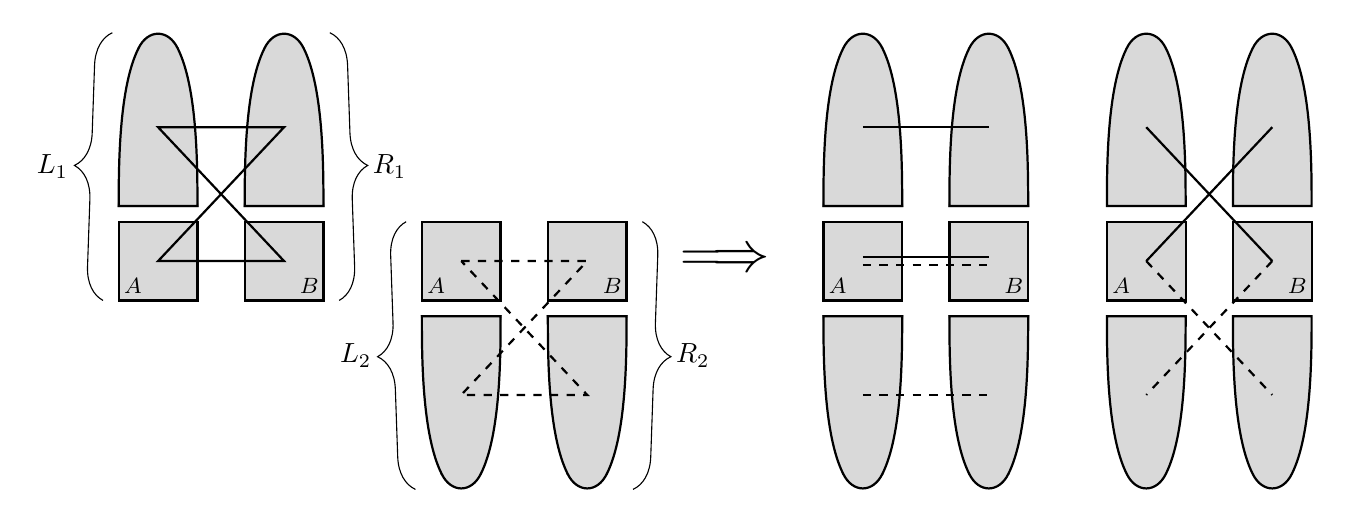
\begin{tikzpicture}

% Command for creating top shape. First 4 arguments expect
% 4 vertices of the form:
% 	(x,y), (x+.25,y+2), (x+.75,y+2), (x+1,y) 
% The 5th argument is the outline color, and the 6th
% argument is the fill color.
\newcommand{\mytop}[6]{
\draw[thick, color=#5, fill=#6] (#1) .. controls ($(#1)+(0,.5)$) and ($(#1)+(0,1.5)$) .. (#2) .. controls ($(#2)+(.12,.25)$) and ($(#3)+(-.12,.25)$) .. (#3) .. controls ($(#4)+(0,1.5)$) and ($(#4)+(0,.5)$) .. (#4) -- cycle;
}

% Command for creating bottom shape. First 4 arguments
% expect 4 vertices of the form:
% 	(x,y), (x+.25,y-2), (x+.75,y-2), (x+1,y) 
% The 5th argument is the outline color, and the 6th
% argument is the fill color.
\newcommand{\mybottom}[6]{
\draw[thick, color=#5, fill=#6] (#1) .. controls ($(#1)+(0,-.5)$) and ($(#1)+(0,-1.5)$) .. (#2) .. controls ($(#2)+(.12,-.25)$) and ($(#3)+(-.12,-.25)$) .. (#3) .. controls ($(#4)+(0,-1.5)$) and ($(#4)+(0,-.5)$) .. (#4) -- cycle;
}

% helping polygon 1
\draw[thick, gray] (0,0)node(A1){} -- ($(A1.center)+(.25,2)$)node(A2){} -- ($(A2.center)+(.5,0)$)node(A3){} -- ($(A1.center)+(1,0)$)node(A4){} -- cycle;

% top shape 1
\mytop{A1.center}{A2.center}{A3.center}{A4.center}{black}{gray!30};

% middle 1
\draw[thick, fill=gray!30] ($(A1.center) + (0,-1.2)$)[]node(B1){} rectangle ($(B1.center) + (1,1)$)node(B2){};
\node at ($(B1.north east)+(.05,.05)$) {\footnotesize $A$};

% helping polygon 2
\draw[thick, gray] ($(A4.center)+(.6,0)$)node(C1){} -- ($(C1.center)+(.25,2)$)node(C2){} -- ($(C2.center)+(.5,0)$)node(C3){} -- ($(C1.center)+(1,0)$)node(C4){} -- cycle;

% top shape 2
\mytop{C1.center}{C2.center}{C3.center}{C4.center}{black}{gray!30};

% middle 2
\draw[thick, fill=gray!30] ($(C1.center)+(0,-.2)$)node(D1){} rectangle ($(D1.center)+(1,-1)$)node[](D2){};
\node at ($(D2.north west)+(-.05,.05)$) {\footnotesize $B$};

% fit boxes to center edges
\node[fit=(A1)(A2)(A3)(A4)] (top1){};
\node[fit=(B1)(B2)] (mid1){};
\node[fit=(C1)(C2)(C3)(C4)] (top2){};
\node[fit=(D1)(D2)] (mid2){};

\draw[decorate, decoration={brace, amplitude=12pt}] ($(B1.center)+(-.2,0)$) -- ($(A2.west)+(-.2,.2)$) node[black,midway, xshift=-7mm] {$L_1$};

\draw[decorate,decoration={brace,amplitude=12pt, mirror}] ($(D2.center)+(.2,0)$) -- ($(C3.east)+(.2,.2)$) node[black,midway, xshift=7mm] {$R_1$};

% edges for top {1,2} and middle {1,2}
\draw[thick] (top1.center) -- (top2.center) -- (mid1.center) -- (mid2.center) -- cycle;

% middle 3
\draw[thick, fill=gray!30] ($(D2.center)+(1.25,0)$)node(E1){} rectangle ($(E1.center)+(1,1)$)node(E2){};
\node at ($(E1.north east)+(.05,.05)$) {\footnotesize $A$};

% helping polygon 3
\draw[thick, gray] ($(E1.center)+(0,-.2)$)node(F1){} -- ($(F1.center)+(.25,-2)$)node(F2){} -- ($(F2.center)+(.5,0)$)node(F3){} -- ($(F1.center)+(1,0)$)node(F4){} -- cycle;

% bottom 1
\mybottom{F1.center}{F2.center}{F3.center}{F4.center}{black}{gray!30};

% middle 4
\draw[thick, fill=gray!30] ($(E2.center)+(.6,0)$) node(G1){} rectangle ($(G1.center)+(1,-1)$) node(G2){};
\node at ($(G2.north west)+(-.05,.05)$) {\footnotesize $B$};

% helping polygon 4
\draw[thick,gray] ($(G1.center)+(0,-1.2)$)node(H1){} -- ($(H1.center)+(.25,-2)$)node(H2){} -- ($(H2.center)+(.5,0)$)node(H3){} -- ($(H1.center)+(1,0)$)node(H4){} -- cycle;

% bottom 2
\mybottom{H1.center}{H2.center}{H3.center}{H4.center}{black}{gray!30};

% fit boxes to center edges
\node[fit=(E1)(E2)] (mid3){};
\node[fit=(F1)(F2)(F3)(F4)] (bot1){};
\node[fit=(G1)(G2)] (mid4){};
\node[fit=(H1)(H2)(H3)(H4)] (bot2){};

\draw[decorate, decoration={brace, amplitude=12pt,mirror}] ($(E1.center)+(-.2,1)$) -- ($(F2.west)+(-.2,-.2)$) node[black,midway, xshift=-7mm] {$L_2$};

\draw[decorate,decoration={brace,amplitude=12pt}] ($(G2.center)+(.2,1)$) -- ($(H3.east)+(.2,-.2)$) node[black,midway, xshift=7mm] {$R_2$};

% edges for bottom {1,2} and middle {3,4}
\draw[thick, dashed] (mid3.center) -- (mid4.center) -- (bot1.center) -- (bot2.center) -- cycle;

%%% whole 1
%% middle
\draw[thick, fill=gray!30] ($(G2.center)+(2.5,0)$)node(I1){} rectangle ($(I1.center)+(1,1)$)node(I2){};
\node at ($(I1.north east)+(.05,.05)$) {\footnotesize $A$};

%% top
% helping polygon
\draw[thick, gray] ($(I1.center)+(0,1.2)$)node(J1){} -- ($(J1.center)+(.25,2)$)node(J2){} -- ($(J2.center)+(.5,0)$)node(J3){} -- ($(J1.center)+(1,0)$)node(J4){} -- cycle;

% region
\mytop{J1.center}{J2.center}{J3.center}{J4.center}{black}{gray!30};

%% bottom
% helping polygon
\draw[thick,gray] ($(I1.center)+(0,-.2)$)node(K1){} -- ($(K1.center)+(.25,-2)$)node(K2){} -- ($(K2.center)+(.5,0)$)node(K3){} -- ($(K1.center)+(1,0)$)node(K4){} -- cycle;

% region
\mybottom{K1.center}{K2.center}{K3.center}{K4.center}{black}{gray!30}

%%% whole 2
%% middle
\draw[thick, fill=gray!30] ($(I2.center)+(.6,0)$)node(L1){} rectangle ($(L1.center)+(1,-1)$)node(L2){};
\node at ($(L2.north west)+(-.05,.05)$) {\footnotesize $B$};

%% top
% helping polygon
\draw[thick,gray] ($(L1.center)+(0,0.2)$)node(M1){} --
($(M1.center)+(.25,2)$)node(M2){} -- ($(M2.center)+(0.5,0)$)node(M3){} -- ($(M1.center)+(1,0)$)node(M4){} -- cycle;

% region
\mytop{M1.center}{M2.center}{M3.center}{M4.center}{black}{gray!30};

%% bottom
% helping polygon
\draw[thick,gray] ($(L1.center)+(0,-1.2)$)node(N1){} --
($(N1.center)+(.25,-2)$)node(N2){} -- ($(N2.center)+(0.5,0)$)node(N3){} -- ($(N1.center)+(1,0)$)node(N4){} -- cycle;

% region
\mybottom{N1.center}{N2.center}{N3.center}{N4.center}{black}{gray!30}

%%% fit boxes for whole 1 and whole 2
\node[fit=(J1)(J2)(J3)(J4)] (wt1) {};
\node[fit=(M1)(M2)(M3)(M4)] (wt2) {};
\node[fit=(I1)(I2)] (wm1) {};
\node[fit=(L1)(L2)] (wm2) {};
\node[fit=(K1)(K2)(K3)(K4)] (wb1) {};
\node[fit=(N1)(N2)(N3)(N4)] (wb2) {};

%%% edges for whole 1 and whole 2
\draw[thick] (wt1.center) -- (wt2.center);
\draw[thick] ($(wm1.center)+(0,.05)$) -- ($(wm2.center)+(0,.05)$);
\draw[thick, dashed] ($(wm1.center)+(0,-.05)$) -- ($(wm2.center)+(0,-.05)$);
\draw[thick, dashed] (wb1.center) -- (wb2.center);

%%% whole 3
%% middle
\draw[thick, fill=gray!30] ($(L2.center)+(1,0)$)node(O1){} rectangle ($(O1.center)+(1,1)$)node(O2){};
\node at ($(O1.north east)+(.05,.05)$) {\footnotesize $A$};

%% top
% helping polygon
\node at ($(O1.center)+(0,1.2)$) (P1){};
\node at ($(P1.center)+(0.25,2)$) (P2) {};
\node at ($(P2.center)+(.5,0)$) (P3) {};
\node at ($(P1.center)+(1,0)$) (P4) {};

% region
\mytop{P1.center}{P2.center}{P3.center}{P4.center}{black}{gray!30};

%% bottom
% helping polygon
\node at ($(O1.center)+(0,-.2)$) (Q1){};
\node at ($(Q1.center)+(.25,-2)$) (Q2){};
\node at ($(Q2.center)+(0.5,0)$) (Q3){};
\node at ($(Q1.center)+(1,0)$) (Q4){};

% region
\mybottom{Q1.center}{Q2.center}{Q3.center}{Q4.center}{black}{gray!30}

%%% whole 4
%% middle
\draw[thick, fill=gray!30] ($(O2.center)+(0.6,0)$)node(R1){} rectangle ($(R1.center)+(1,-1)$)node(R2){};
\node at ($(R2.north west)+(-.05,.05)$){\footnotesize $B$};

%% top
% helping nodes
\node at ($(R1.center)+(0,.2)$) (S1){};
\node at ($(S1.center)+(.25,2)$) (S2){};
\node at ($(S2.center)+(.5,0)$) (S3){};
\node at ($(S1.center)+(1,0)$) (S4){};

% region
\mytop{S1.center}{S2.center}{S3.center}{S4.center}{black}{gray!30};

%% bottom
% helping nodes
\node at ($(R1.center)+(0,-1.2)$) (T1){};
\node at ($(T1.center)+(.25,-2)$) (T2){};
\node at ($(T2.center)+(.5,0)$) (T3){};
\node at ($(T1.center)+(1,0)$) (T4){};

% region
\mybottom{T1.center}{T2.center}{T3.center}{T4.center}{black}{gray!30};

%%% fit boxes for whole 3 and 4
\node[fit=(P1)(P2)(P3)(P4)] (wt3){};
\node[fit=(S1)(S2)(S3)(S4)] (wt4){};
\node[fit=(O1)(O2)] (wm3){};
\node[fit=(R1)(R2)] (wm4){};
\node[fit=(Q1)(Q2)(Q3)(Q4)] (wb3){};
\node[fit=(T1)(T2)(T3)(T4)] (wb4){};

%%% edges for whole 3 and 4
\draw[thick] (wt3.center) -- (wm4.center) (wt4.center) -- (wm3.center);
\draw[thick,dashed] (wm3.center) -- (wb4.center) (wm4.center) -- (wb3.center);

%%% middle implies
\node at ($(mid4.center)!0.5!(wm1.center)$) {\huge$\implies$};

\end{tikzpicture}
\end{center}
\caption{General outline of how our algorithm proceeds at each step.}
\end{figure}

\newpage
\appendix


\end{document}
